\setcounter{framenumber}{0}
%35


\begin{frame}
  \titlepage
\end{frame}

\begin{frame}{Learning Goals}
By the end of this lecture, students should be able to:

\begin{itemize}
    \item state the axioms of probability;
    \item understand probability as a mathematical function on events;
    \item derive basic consequences of the axioms;
    \item apply the addition rule;
    \item use complements and inclusion--exclusion;
    \item identify mutually exclusive events;
    \item understand why axiomatic probability generalizes naive probability.
\end{itemize}
\end{frame}

\lecturepart{Why Axiomatize Probability (or anything)?}

\begin{frame}{Limitations of Naive Probability}
Previously, we defined (naive) probability by

\[
\Prob(A)=\frac{|A|}{|\Sample|}.
\]

This works well when:
\begin{itemize}
    \item the sample space is finite;
    \item all outcomes are equally likely.
\end{itemize}

\vspace{0.3cm}

But many important situations do not satisfy these assumptions.

\vspace{0.25cm}

Examples:
\begin{itemize}
    \item infinitely many outcomes;
    \item continuous measurements;
    \item unequal likelihoods;
    \item etc.
\end{itemize}
\end{frame}

\begin{frame}{The Axiomatic Point of View}
Instead of defining probability by counting, we define probability abstractly using properties that probabilities should satisfy.

\vspace{0.3cm}

\begin{keybox}{Idea}
A probability measure assigns a number to each event:
\[
A \longmapsto \Prob(A),
\]
subject to certain axioms (i.e., principles, rules) .
\end{keybox}

\vspace{0.3cm}

The naive definition will become a special case of the general theory.
\end{frame}

\lecturepart{The Axioms of Probability}

\begin{frame}{Probability Space}
A probability model consists of:

\begin{enumerate}
    \item $\Sample$: sample space  (set of all possible outcomes in an experiment);
    \item $\mathcal{F} $: a collection of subsets of $\Sample$ (aka "events") ;
    \item $\mathbb{P}(\cdot)$: a probability function $\Prob: \mathcal{F}\to [0,1]$.
\end{enumerate}

\vspace{0.25cm}

So for any event $A\subseteq \Sample$ (or $A\in \mathcal{F})$, $\mathbb{P}(A)$ is the probability that the function $\mathbb{P}(\cdot)$ assigns to $A$.



These 3 elements together form a Probability Model:
$$(\Sample , \mathcal{F}, \mathbb{P})$$

Note that the probability function assigns numbers to sets (events), not to numbers (this might be new for us). So we will see things like $\mathbb{P}([1,2])$, $\mathbb{P}((-\infty, 4])$, or $\mathbb{P}(\{ 2,4,6\} )$

\end{frame}

\begin{frame}{Axiom 1: Nonnegativity}
\begin{keybox}{Axiom 1}
For every event $A\subseteq \Sample$,
\[
\boxed{\Prob(A)\geq0.}
\]
\end{keybox}

\vspace{0.3cm}

Interpretations:
\begin{itemize}
    \item probabilities cannot be negative;
    \item impossible events have probability $0$;
    \item larger probabilities correspond to more likely events.
\end{itemize}
\end{frame}

\begin{frame}{Axiom 2: Normalization}
\begin{keybox}{Axiom 2}
The probability that "something happens", is $1$:
\[
\boxed{\Prob(\Sample)=1.}
\]
In other words, $\mathbb{P}(\cdot)$ assigns the number $1$ to the event $\Sample \in \mathcal{F}$.
\end{keybox}

\end{frame}

\begin{frame}{Axiom 3: Additivity}
\begin{keybox}{Axiom 3}
If
\[
A_1,A_2,A_3,\dots
\]
are pairwise disjoint events, then

\[
\boxed{
\Prob\left(\bigcup_{i=1}^{\infty} A_i\right)
=
\sum_{i=1}^{\infty}\Prob(A_i).
}
\]
\end{keybox}

\vspace{0.25cm}

Pairwise disjoint means:
\[
A_i \cap A_j = \emptyset
\qquad \text{whenever } i\neq j.
\]
\end{frame}

\begin{frame}{Finite Additivity}
Axiom 3 immediately implies the finite version:

If
\[
A_1,\dots,A_n
\]
are disjoint, then

\[
\Prob(A_1\cup\cdots\cup A_n)
=
\Prob(A_1)+\cdots+\Prob(A_n).
\]

\vspace{0.3cm}

In particular, if
\[
A\cap B=\emptyset,
\]
then

\[
\boxed{
\Prob(A\cup B)=\Prob(A)+\Prob(B).
}
\]
\end{frame}

\lecturepart{Basic Consequences of the Axioms}

\begin{frame}{Probability of the Empty Set}
\begin{keybox}{Proposition}
\[
\Prob(\emptyset)=0.
\]
\end{keybox}

\vspace{0.25cm}

Reason:

\[
\Sample = \Sample \cup \emptyset,
\]
and
\[
\Sample \cap \emptyset=\emptyset.
\]

Using additivity,

\[
\Prob(\Sample)
=
\Prob(\Sample)+\Prob(\emptyset).
\]

Since $\Prob(\Sample)=1,$ we obtain ${\Prob(\emptyset)=0.}
$
\end{frame}

\begin{frame}{Complements}
\begin{keybox}{Proposition (Complement Rule)}
For every event $A$,
\[
\boxed{
\Prob(A^c)=1-\Prob(A).
}
\]
\end{keybox}

\vspace{0.25cm}

Reason:

\[
A\cup A^c=\Sample,
\]
and
\[
A\cap A^c=\emptyset.
\]

Thus,

\[
1
=
\Prob(\Sample)
=
\Prob(A)+\Prob(A^c).
\]
\end{frame}

\begin{frame}{Probabilities Are Between 0 and 1}
\begin{keybox}{Proposition}
For every event $A$,
\[
0\leq \Prob(A)\leq1.
\]
\end{keybox}

\vspace{0.25cm}

Why?

\vspace{0.2cm}

Axiom 1 gives:
\[
\Prob(A)\geq0.
\]

Also,
\[
\Prob(A^c)\geq0.
\]

Using
\[
\Prob(A^c)=1-\Prob(A),
\]
we obtain
\[
1-\Prob(A)\geq0
\]
\end{frame}

\begin{frame}{Monotonicity} \begin{keybox}{Proposition (Monotonicity)} For any event $A,B\subseteq \Sample$ if $A\subseteq B,$ then \[ \boxed{ \Prob(A)\leq \Prob(B). } \] \end{keybox} \vspace{0.25cm} 

\begin{proof}
If $A\subseteq B,$ then $B=A\cup(B\setminus A),$ where the two events ($A$ and $B-A$) are disjoint (why?). 
\vspace{3mm}
Thus, 
\begin{equation*}
    \Prob(B) = \Prob(A)+\Prob(B\setminus A)\geq\Prob(A),
\end{equation*}
since $\mathbb{P}(B-A)\geq 0$ according to Axiom 1. 
\end{proof}




\end{frame}


\begin{frame}{Monotonicity: Picture}

\begin{center}
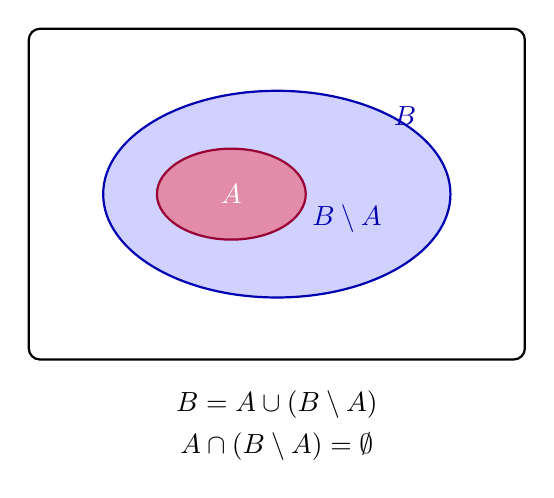
\begin{tikzpicture}[scale=1.05]

% Sample space
\draw[thick, rounded corners] (-3,-2) rectangle (3,2);
\node at (2.45,1.65) {$\Sample$};

% B
\fill[blue!18] (0,0) ellipse (2.1 and 1.25);
\draw[blue!70!black, thick] (0,0) ellipse (2.1 and 1.25);
\node[blue!70!black] at (1.55,0.95) {$B$};

% A
\fill[purple!45] (-0.55,0) ellipse (0.9 and 0.55);
\draw[purple!80!black, thick] (-0.55,0) ellipse (0.9 and 0.55);
\node[white] at (-0.55,0) {$A$};

% B minus A label
\node[blue!70!black] at (0.85,-0.3) {$B\setminus A$};

% Formula under diagram
\node at (0,-2.55) {$B=A\cup(B\setminus A)$};
\node at (0,-3.05) {$A\cap(B\setminus A)=\emptyset$};

\end{tikzpicture}
\end{center}

\vspace{0.15cm}

\begin{center}
Since $B$ contains all of $A$ plus the extra part $B\setminus A$,
\[
\Prob(B)=\Prob(A)+\Prob(B\setminus A)\geq \Prob(A).
\]
\end{center}

\end{frame}










\lecturepart{The Addition Rule}

\begin{frame}{Why Finite Additivity Is Not Enough}
Suppose $A$ and $B$ are not disjoint.

Then:

\[
\Prob(A\cup B)
\neq
\Prob(A)+\Prob(B).
\]

Why?

\vspace{0.2cm}

Because outcomes in
\[
A\cap B
\]
are counted twice.
\end{frame}

\begin{frame}{The Addition Rule}
\begin{keybox}{Proposition:  Addition Rule}
For any events $A$ and $B$,
\[
\boxed{
\Prob(A\cup B)
=
\Prob(A)+\Prob(B)-\Prob(A\cap B).
}
\]
\end{keybox}


\begin{proof}
    Partition $A\cup B$ into three disjoint subsets and use a similar trick that was appkied to prove Monotonicity previously.
\end{proof}




\end{frame}

\begin{frame}{Why the Addition Rule Works}
When adding
\[
\Prob(A)+\Prob(B),
\]
outcomes in
\[
A\cap B
\]
are counted twice.

\vspace{0.25cm}

Therefore we subtract one copy:

\[
\Prob(A\cup B)
=
\Prob(A)+\Prob(B)-\Prob(A\cap B).
\]
\end{frame}


\begin{frame}{Mutually Exclusive Events}
\begin{keybox}{Definition}
Events $A$ and $B$ are called \textbf{mutually exclusive} (or disjoint) if
\[
A\cap B=\emptyset.
\]
\end{keybox}

\vspace{0.25cm}

In that case,
\[
\Prob(A\cap B)=0,
\]
so the addition rule becomes:

\[
\Prob(A\cup B)
=
\Prob(A)+\Prob(B).
\]
\end{frame}

\begin{frame}{Example: Die Roll}
Roll one fair die.

Let
\[
A=\{\text{roll is even}\}=\{2,4,6\},
\]
\[
B=\{\text{roll is odd}\}=\{1,3,5\}.
\]

Then
\[
A\cap B=\emptyset.
\]

Thus
\[
\Prob(A\cup B)
=
\Prob(A)+\Prob(B).
\]

Indeed,
\[
\frac12+\frac12=1.
\]
\end{frame}

\lecturepart{Inclusion--Exclusion}

\begin{frame}{Three-Set Inclusion--Exclusion}
For three events:

\[
\Prob(A\cup B\cup C)
\]

we first add:

\[
\Prob(A)+\Prob(B)+\Prob(C).
\]

\vspace{0.25cm}

Then subtract pairwise intersections:

\[
-\Prob(A\cap B)
-\Prob(A\cap C)
-\Prob(B\cap C).
\]

\vspace{0.25cm}

But now the triple intersection has been subtracted too many times, so we add it back.
\end{frame}

\begin{frame}{Inclusion--Exclusion Formula}
\begin{keybox}{Three-Set Inclusion--Exclusion}
\[
\boxed{
\begin{aligned}
\Prob(A\cup B\cup C)
&=
\Prob(A)+\Prob(B)+\Prob(C)
\\
&\quad
-\Prob(A\cap B)
-\Prob(A\cap C)
-\Prob(B\cap C)
\\
&\quad
+\Prob(A\cap B\cap C).
\end{aligned}
}
\]
\end{keybox}
\end{frame}


\lecturepart{Partitions}

\begin{frame}{Partitions of the Sample Space}
\begin{keybox}{Definition}
Events
\[
A_1,\dots,A_n
\]
form a partition of $\Sample$ if:

\begin{enumerate}
    \item
    \[
    A_i\cap A_j=\emptyset
    \qquad (i\neq j),
    \]

    \item
    \[
    A_1\cup\cdots\cup A_n=\Sample.
    \]
\end{enumerate}
\end{keybox}

\vspace{0.25cm}

A partition divides the sample space into non-overlapping pieces.
\end{frame}











\begin{frame}{Probability of a Partition}
If
\[
A_1,\dots,A_n
\]
form a partition of $\Sample$, then

\[
\boxed{
\Prob(A_1)+\cdots+\Prob(A_n)=1.
}
\]

\vspace{0.25cm}

Reason:

The events are disjoint and their union is $\Sample$.
\end{frame}

\lecturepart{Naive Probability as a Special Case}

\begin{frame}{Recovering Naive Probability}
Suppose:
\begin{itemize}
    \item $\Sample$ is finite;
    \item all outcomes are equally likely.
\end{itemize}

Let $\Sample = \{s_1, s_2, \dots ,s_n \} $

Assign equal probability weights to each outcome:
\[
\mathbb{P}(s_1) = \mathbb{P}(s_2) = \dots = \mathbb{P}(s_n) = \frac1n.
\]

Then for an event $A$, we have

\[
\Prob(A) = \Prob (\cup_{s_j\in A} s_j) = \sum_{i \in A}\frac{1}{n} =
|A| \times \frac{1}{n}
=
\frac{|A|}{|\Sample|}.
\]

\vspace{0.25cm}

Thus the naive definition satisfies the probability axioms.
\end{frame}

\begin{frame}{Mini-Exercises}
\begin{enumerate}
    \item If
    \[
    \Prob(A)=0.3,
    \]
    what is
    \[
    \Prob(A^c)?
    \]

    \item If
    \[
    \Prob(A)=0.6,
    \qquad
    \Prob(B)=0.5,
    \qquad
    \Prob(A\cap B)=0.1,
    \]
    compute
    \[
    \Prob(A\cup B).
    \]

    \item Can two disjoint events both have probability $1$?

\end{enumerate}

\begin{livebox}{Answers}
\[
0.7,
\qquad
1.0.
\]
\end{livebox}
\end{frame}

\begin{frame}{Summary}
\begin{itemize}
    \item Probability is defined axiomatically.

    \item The axioms are:
    \[
    \Prob(A)\geq0,
    \qquad
    \Prob(\Sample)=1,
    \]
    and countable additivity.

    \item Important consequences include:
    \[
    \Prob(\emptyset)=0,
    \qquad
    \Prob(A^c)=1-\Prob(A),
    \qquad 
    0\leq\Prob(A)\leq1.
    \]

    \item The addition rule is:
    \[
    \Prob(A\cup B)
    =
    \Prob(A)+\Prob(B)-\Prob(A\cap B).
    \]

    \item Naive probability is a special case of axiomatic probability.
\end{itemize}

\vspace{0.25cm}

\begin{keybox}{Next lecture}
Conditional probability and independence.
\end{keybox}
\end{frame}